
\documentclass[onehalf,11pt]{beavtex}
\title{Activity Detection on Free-Living Data Using Change-Point Detection}
\author{Michael M. Anderson}
\degree{Master of Science}
\doctype{Thesis}
\department{Electrical Engineering and Computer Science}
\depttype{School}
\depthead{Director}
\major{Computer Science}
\advisor{Weng-Keen Wong}
\submitdate{June 13, 2013}
\commencementyear{2013}

\usepackage{amsmath}
\usepackage{graphicx}
\usepackage{mathtools}
\usepackage{epstopdf}
\usepackage{multirow}
\usepackage{caption}
\usepackage{float}
\usepackage{subfigure}
\graphicspath{ {figures/} }
%\graphicspath{ {results/} }

%\usepackage{algorithm}
%\usepackage{algorithmic}
%\usepackage{times}
%\usepackage{courier}
%\usepackage{helvet}

\abstract{
Activity detection on time series sensor data is a rapidly emerging field with
a lot of potential real-world application. In previous work researchers have
unrealistically assumed that they know at which ticks in a time series the
given subject stops doing one activity and starts doing another. In this thesis
we explore the feasibility of segmenting realistic free-living time series data
using techniques from
change-point detection, and then classifying the predicted segments using
standard supervised learning techniques. We compare this to the popular
approach of splitting the time series into small windows of fixed-length,
predicting on each window with a classifier, and then smoothing over the
predictions with an HMM. We find that the HMM approach clearly outperforms the
change-point detection approach, but that change-point detection may be
promising given a modeling assumption that is appropriate to the data.
}

\acknowledgements{
I would like to acknowledge and thank my advisor, Dr. Weng-Keen Wong, for
providing me with a clear and overarching vision of this project at all stages of its
development, as well as his general expertise and helpfulness with all of the
rough patches, sticking points, and unexpected problems that invariably
accompany an endeavor of this magnitude. I would also like to thank the
other members of my committee, Dr. Alan Fern, Dr. Raviv Raich, and Dr. Hector
Vergara, for giving their time to help supervise the final stages of this
project. Thanks go to all of my family and friends who encouraged and stood by
me along the way. They are too numerous to name but they know who they are.
}

\begin{document}
\maketitle
\mainmatter

%I have done some excellent research \cite{matrix}.
%\begin{figure}[!ht]
%\centering
%\fbox{\huge Box}
%\caption{Go figure.}
%\end{figure}

\chapter{Introduction}
One of the general goals of artificial intelligence is to build
computing devices that are ``context-aware'', that act as
more than just passive number-crunching machines that receive input data through very
restrictive and wholly human-operated channels such as a keyboard or mouse.
Context-aware devices are capable of using sensor data to understand the
environment that they are situated in, such as the locations of nearby objects
and how the objects are moving \cite{abowd99}. One subfield of context-aware
computing that has been receiving considerable attention in recent years is activity
detection. The goal of activity detection is to build computer plus sensor systems
that are able to determine what activity a human subject is performing at any given
moment.

Such systems have a variety of real-world applications. Research is 
exploring the feasibility of using both wearable and non-wearable sensor systems to
monitor the health of elderly patients that have or are at risk of developing
degenerative physical and mental diseases \cite{fogarty06}. The goal is to 
build sensor-based monitoring systems that can aid doctors and family
members in tracking the decline of patients over time. Also, detection of an
abnormal activity may indicate that a senior is undergoing a serious medical
event such as a heart attack or slip-and-fall \cite{wang12}.
Another application of activity detection is to track the energy expenditure
of subjects as they go through the course of their day. The
traditional method of performing such tracking is with self-reporting by the
subject of their activities. Wearable sensors offer an alternative approach that
is not susceptible to misreporting due to bias, poor memory, or other
confounding factors that a human reporter introduces into the system. One
approach is to use sensor data to estimate the vigorousness or metabolic equivalent
(MET) of an activity and calculate energy expenditure directly \cite{staudenmeyer09},
while another is to attempt to predict the type of activity performed, and calculate energy
expenditure using knowledge of how vigorous that activity is generally \cite{trost12}.

Activity detection generally assumes that sensor data will be represented as a
time series, and that at any given moment in the time series the subject is
performing one and only one type of activity. Thus the time series is thought
of as being partitioned into a number of non-overlapping intervals (\emph{windows}), which are
delimited by moments in time when the subject stopped performing one activity
and started performing another. Previous work has treated activity detection as an
offline problem, and has rarely considered performance metrics other than accuracy.
In this work we are interested in the feasibility of partitioning and
classifying a time series on free-living data in real time. In addition to
accuracy, we will also evaluate our algorithms in terms of the amount of time
required to detect that an activity change has occurred.

We used change-point detection to partition time series data into activity windows for classification.
Change-point detection is a field of statistics popular in control theory and other similar
applications. We call this our top-down approach, because this
method takes as input an initial time series and partitions it into smaller pieces using
change-point detection. As an alternate approach we
used the well-known technique of partitioning the time series into small fixed-length,
non-overlapping windows, predicting the activity type of each window
using a base classifier, treating that prediction as the observable
state of an HMM, and then finally solving the HMM for its hidden states. We call
this our bottom-up approach, because we begin with small windows of fixed-length,
and use an HMM to smooth windows together into larger activity intervals.

\chapter{Related Work}
As mentioned in the previous chapter, sensor systems may consist
of environmental or wearable devices. Some examples of environmental
sensors that activity detection researchers have used to
gather data are microphones \cite{fogarty06}, weight detection
panels \cite{rowan05}, cameras \cite{duong05}, and water usage detectors
\cite{fogarty06}. Researchers will generally place environmental sensors
inside of a house, have subjects live in the house for a period of time, and
attempt to predict for activity types like cooking, watching TV, etc.

Various wearable devices have been tried as well, such as RFID gloves
\cite{gu09} \cite{rowan05}, but the most popular wearable for activity detection
purposes is the accelerometer. Besides being inexpensive, accelerometers
tend to be small and lightweight, and so are fairly unobtrusive and
user-friendly. Accelerometers also gather data at a high frequency, and as such
may be used to collect a sizeable amount of data in a relatively short amount
of time.

Whether or not an accelerometer will be discriminative for a
set of activity types depends partially on where the accelerometer is worn on
a subject's body. For example, an accelerometer worn on the ankle will be
more discriminative for the activity of cycling than it would be if it was worn
on the hip, and different types of arm movements will likely be
discriminated only by an accelerometer worn on the arm. For this reason some
researchers have opted to use multiple accelerometer systems to capture
movement information from different parts of the body \cite{bao04}
\cite{devries11}. However, this approach can be cumbersome for the wearer, so a
single accelerometer is preferred when it is reasonable to assume that it will
be discriminative over the relevant set of activities. Further research has
leveraged the accelerometers found in smart phones that subjects
are likely to carry with them anyway as data collection devices
\cite{bao04} \cite{choudhury08} \cite{kwapitz10}

Activity sensor data tends to be noisy and not amenable to a
deterministic or rule-based analysis, so activity types are typically modeled
probabilistically, and activity detection is usually formulated as a supervised
learning problem. The various common supervised learning algorithms are all
familiar to the activity detection literature, though neural networks are
especially popular, such as in \cite{aminian95} \cite{song07} \cite{staudenmeyer09}.
More complicated metamodeling approaches have also been tried, such as
plurality voting with bagged, boosted, and stacked classifiers \cite{ravi05};
conditional random fields \cite{blanke10} \cite{gu09} \cite{vankasteren08} \cite{wu09}; and HMMs
\cite{gu09} \cite{lester05} \cite{pober06} \cite{wu09}.

In the past few years researchers have started to focus on the feasibility of
online activity detection \cite{keogh01} \cite{wu09}, and have started to
recognize the need to test on realistic free-living data \cite{gu09} \cite{kwapitz10}
\cite{strohrmann11}. Our contribution is to compare different change-point detection
techniques for window segmentation with the state-of-the-art (in terms of
accuracy) HMM approach on free-living data in an online setting.

\chapter{Methodology}
\section{Overview}
Each dataset that we tested consisted of multiple time series gathered from
a number of different subjects, so to perform an experiment on a dataset we began by
partitioning the set of time series into disjoint subsets of training, validation,
and test data. Each individual time series was then partitioned into
a set of disjoint windows, and each window was converted into its own feature vector. Once the dataset was
featurized, the experiment could be treated as a typical classification problem.
Base classifiers were built with the training set, and tuned (when necessary)
on the validation set. 
To complete the change-point detection experiments (\ref{fig:cpd_lifecycle}),
the tuned model was evaluated with the testing data. For the HMM experiments
(\ref{fig:hmm_lifecycle}), the tuned model made predictions on a
second training set, which were used to build an HMM metamodel. Finally, that
metamodel was evaluated with the testing data. Following sections describe these
processes in detail.

\begin{figure}
 \centering
 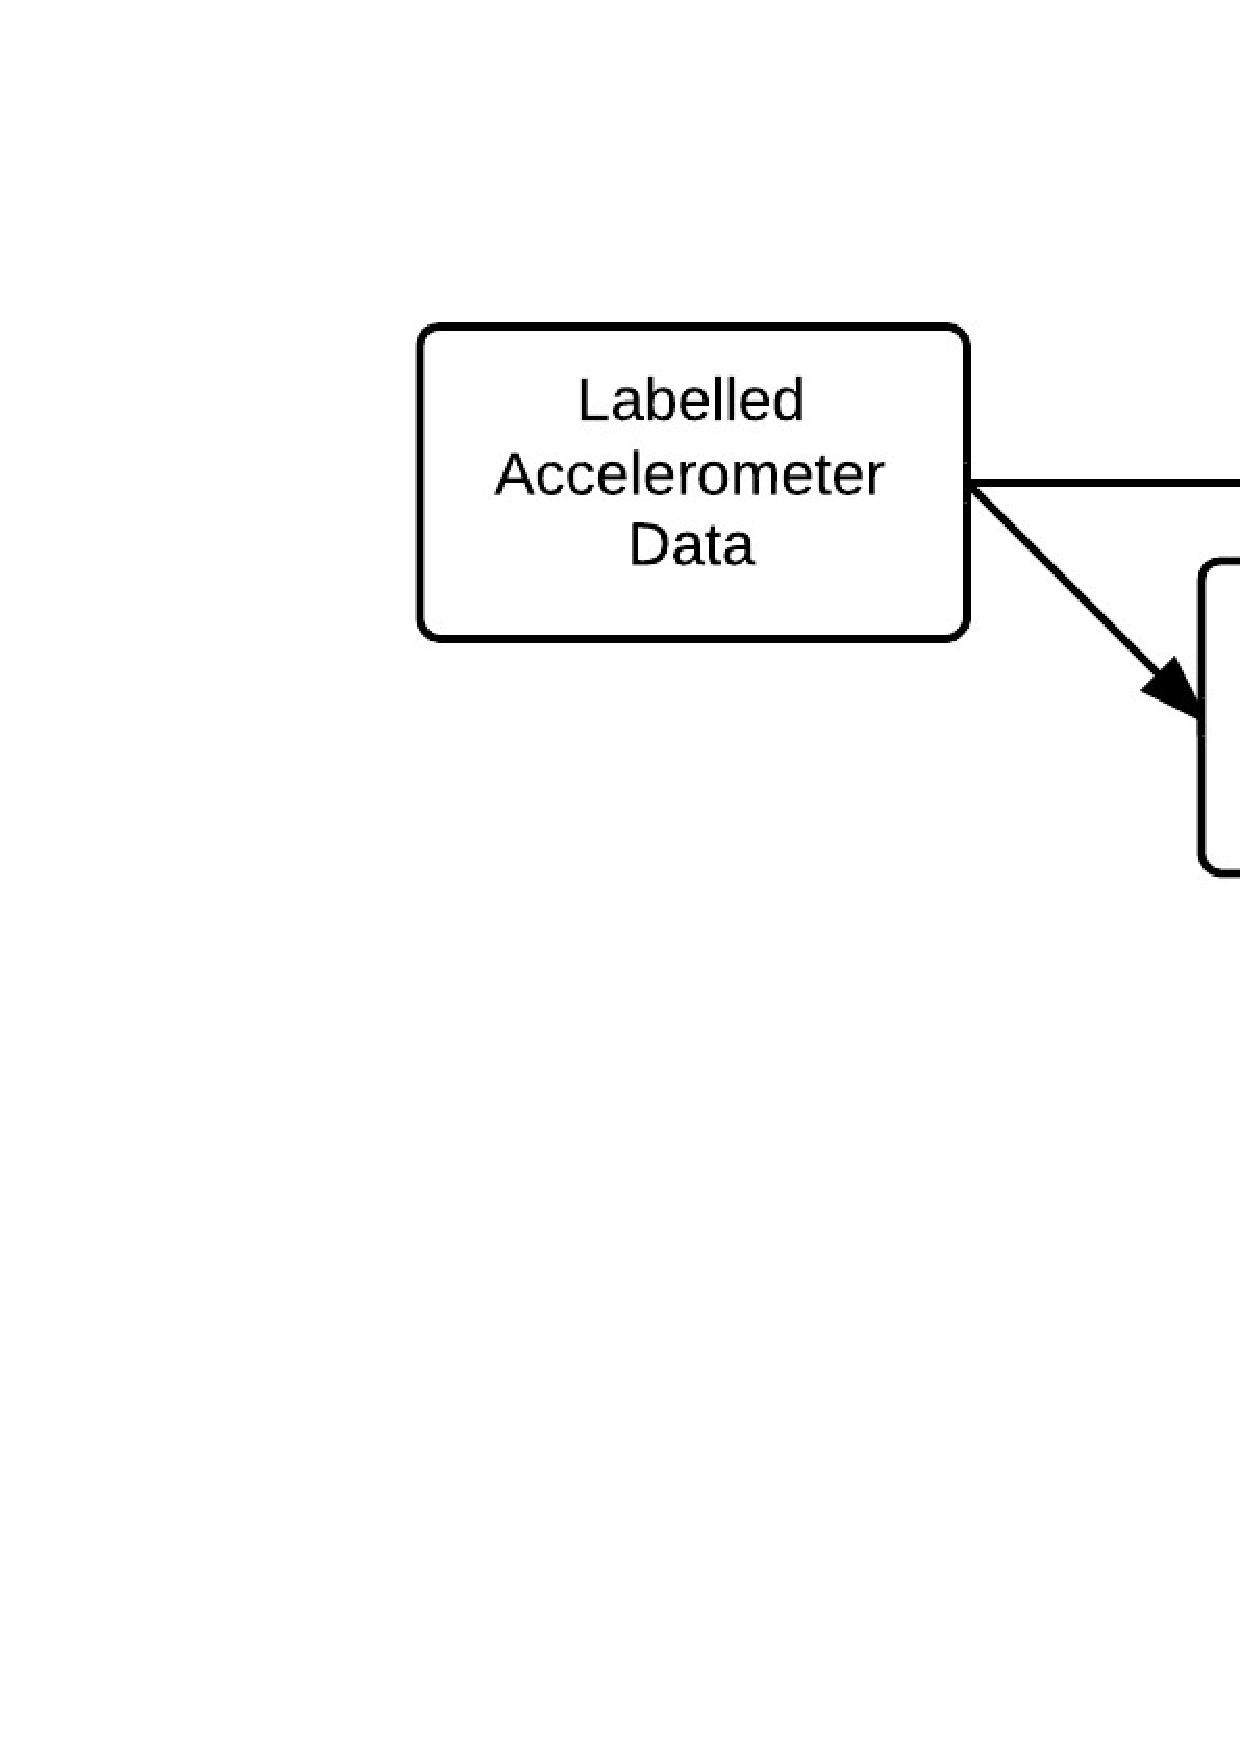
\includegraphics[scale=0.6]{cpd_lifecycle.pdf}
 \caption{Data Lifecycle for Change-Point Detection Experiments}
 \label{fig:cpd_lifecycle}
\end{figure}

\begin{figure}
 \centering
 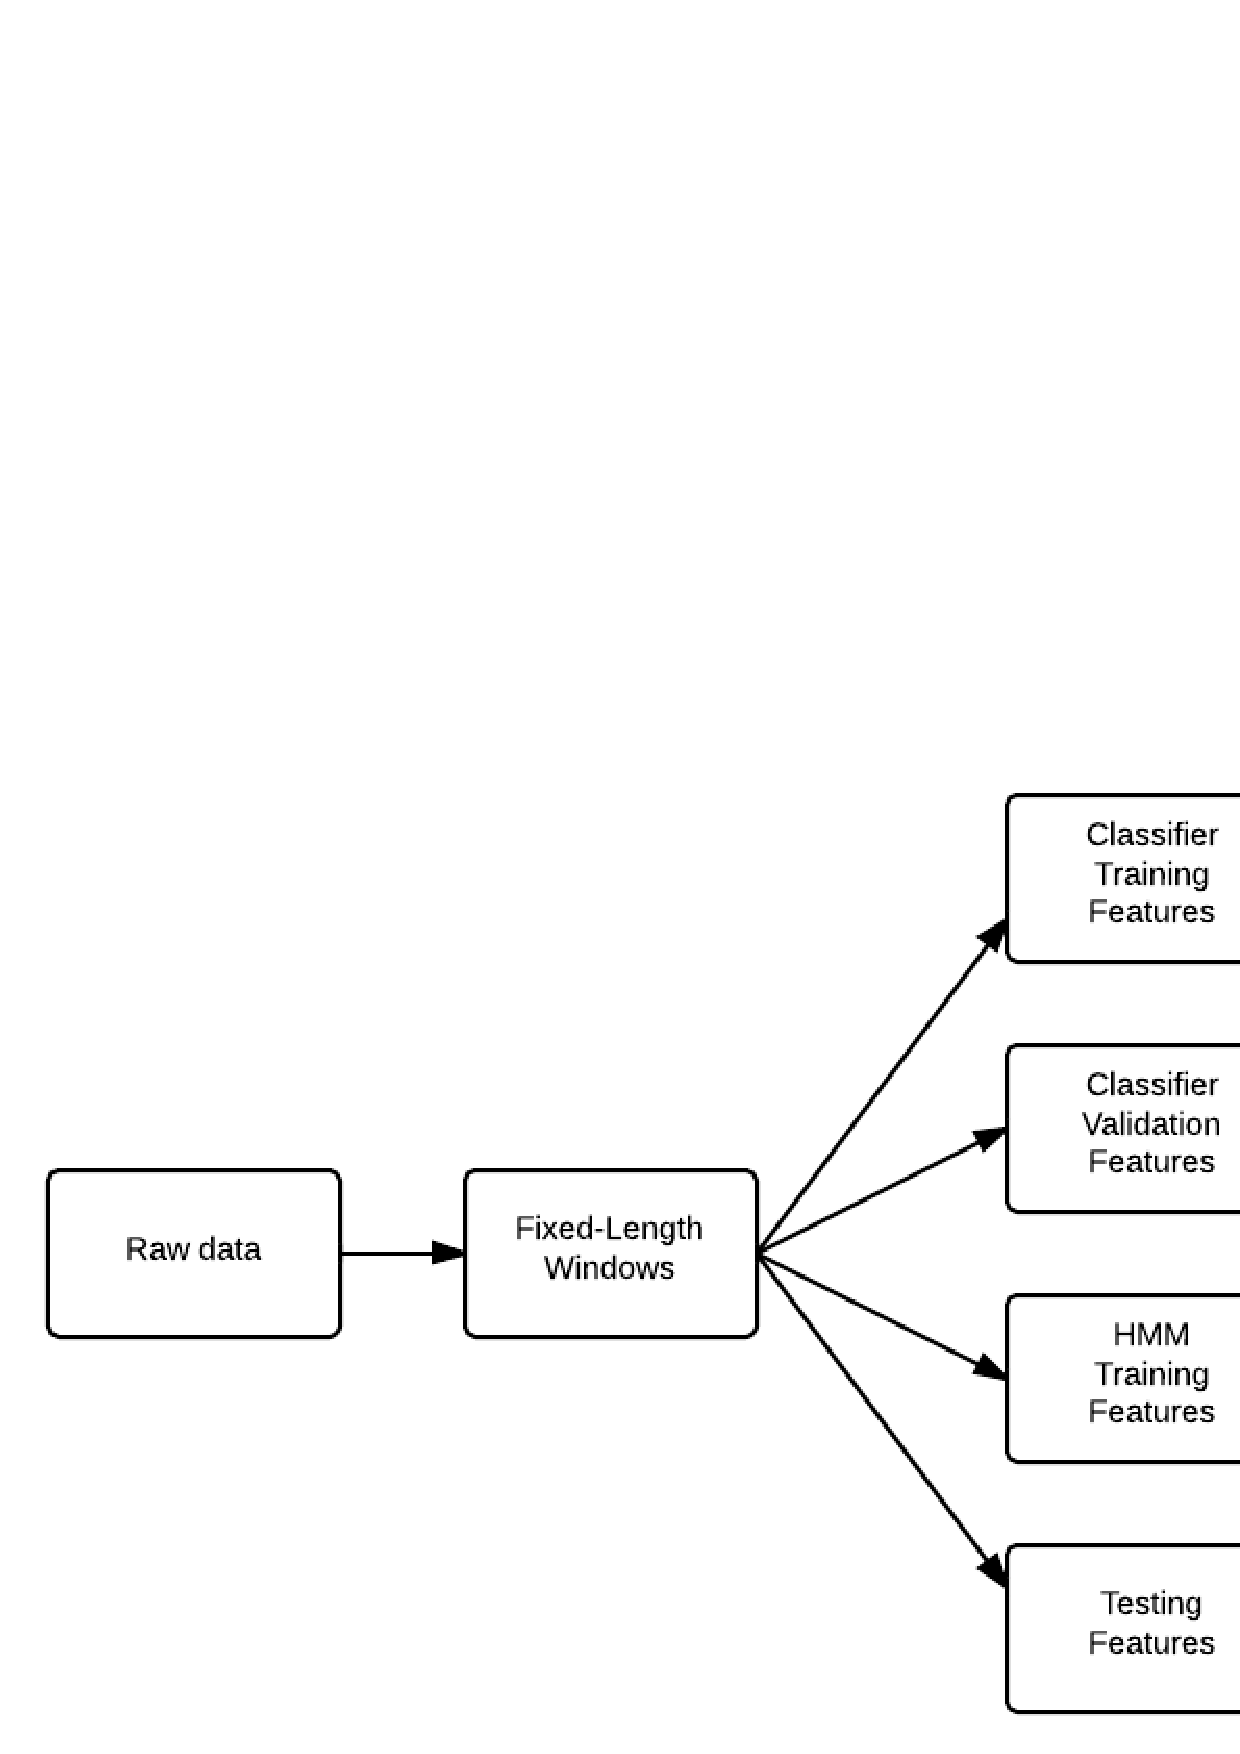
\includegraphics[scale=0.6]{hmm_lifecycle.pdf}
 \caption{Data Lifecycle for HMM Experiments}
 \label{fig:hmm_lifecycle}
\end{figure}

%TODO:Maybe cite example(s) of non-free-living data
\section{Datasets}
For our experiments we were interested in testing our algorithms on real-world free-living
data. In the past, researchers have gathered activity data under unrealistic
laboratory conditions, and by performing activities themselves instead of using
independent subjects.
Unfortunately there are not many such labeled free-living datasets available,
so we only tested our algorithms on two datasets.

\subsection{OSU Hip}
Our first dataset was collected by the Nutrition and Exercise Sciences department of
Oregon State University, and has been used for previous activity detection research
with the goal of designing a system to calculate and monitor subjects' energy expenditure
\cite{trost12} \cite{zheng12}.
This dataset consisted of 91 time series collected over a 2-week period in a
laboratory environment, from 50 subjects who were children between the ages of 5 and 15.
Subjects performed 12 different types of activities (as shown in Figure \ref{fig:osu_activities})
over two separate visits, while an ActiGraph GT1M accelerometer worn on their hip 
collected triaxial acceleration data at a frequency of 30Hz.

Data was collected from two separate visits to the lab, where the subjects performed 6 activities per visit.
The 12 activities were performed in the same order for every other subject.
In the version of the dataset available to us, we had all 12 activities of
41 of the subjects, only the first 6 activities of an additional 5 subjects,
and the last 6 activities of the remaining 4 subjects.
Subjects were given breaks in between each activity and activities lasted 5-10
minutes, however, these unlabelled breaks were removed from the version that we
used. Additionally, only two minutes of data were available for each subject, so 
time series consisted of six 120 second long activities that were concatenated together,
qualifying the data as synthetic. Each of the 91 time series contained a total of
$6*120*30 = 21600$ data ticks.

\begin{figure}
 \centering
 \includegraphics[scale=0.3]{osu_lying.png}
 \includegraphics[scale=0.3]{osu_writing.png}
 \includegraphics[scale=0.3]{osu_laundry.png}
 \includegraphics[scale=0.3]{osu_catch.png}
 \includegraphics[scale=0.3]{osu_comf_walking.png}
 \includegraphics[scale=0.3]{osu_dancing.png}
 \includegraphics[scale=0.3]{osu_computer.png}
 \includegraphics[scale=0.3]{osu_sweeping.png}
 \includegraphics[scale=0.3]{osu_brisk_walking.png}
 \includegraphics[scale=0.3]{osu_basketball.png}
 \includegraphics[scale=0.3]{osu_running.png}
 \includegraphics[scale=0.3]{osu_treadmill.png}
 \caption{OSU Hip Activity Samples}
 \label{fig:osu_activities}
\end{figure}

We determined that several of the activities were very similar and that
it would be difficult to discriminate between them, so we combined some of them together to
create a 7 class version of the data.
Our classes were lying down, sitting (hand-writing, computer game),
standing (laundry, sweeping, and catch), walking (comfortable, brisk and treadmill walking),
dancing, running, and basketball.

\subsection{LiME}
This dataset consisted of 23 time series, each containing roughly 10 continuous
days worth of data from an individual subject. It was collected by Helen Brown from
the Univerity of Cambridge, and Gemma Ryde from the University of Stirling, Scotland.
Subjects wore an ActiGraph GT3X+
accelerometer during the entire period, which collected triaxial acceleration data at a frequency
of 30Hz, as well as an activPal inclinometer on their thighs. The inclinometer
provided what we considered the ground truth labels of the data by automatically
delimitting and classifying intervals using the orientation of the subject's thigh at any given moment. It 
classified a horizontal orientation as lying down/sitting,
a vertical orientation as standing, and a combination of the two as walking. Figure
\ref{fig:lime_activities} shows samples of accelerometer data from the 3 activities.

\begin{figure}
 \centering
 \includegraphics[scale=0.3]{lime_lying.png}
 \includegraphics[scale=0.3]{lime_standing.png}
 \includegraphics[scale=0.3]{lime_walking.png}
 \caption{LiME Day 1 Activity Samples}
 \label{fig:uq_activities}
\end{figure}

This dataset was challenging to work with because of its size, as each individual time series
contained roughly 25 million ticks of data. To help alleviate this problem, we split each
time series into individual days. We then treated the first 24 hour period of data that began at midnight,
from each subject, as one whole dataset (LiME Day 1), and the second such period as a separate dataset
(LiME Day 2). We did not use any data from the remaining days.

In contrast to the OSU Hip dataset, LiME
was not synthetic and activity lengths were variable. For LiME Day 1, the
average activity length was 2977 with a standard deviation of 26428, and the
median length was 348. The average number of activities per time series was
871. As would be expected, statistics for LiME Day 2 were comparable: the
average activity length was 3108 with a standard deviation of 24099, and the
median length was 348. The average number of activities per time series was 834.
The medians were relatively small because many of the activities were short,
while the mean and standard deviations were larger because a few of the
activities were extremely long (when subjects were sleeping, for example).

\section{Featurization}
To formulate our experiments as classification problems, we split each time series into a set of
non-overlapping windows and represented each window as a feature vector.
How we decided where one window ended (and where the next began) varied between
experiments, and is described in sections \ref{sec:topdown} and \ref{sec:bottomup}. Our feature
set was a large collection of statistics that have been shown to be discriminative
for activity classification in previous research \cite{li09} \cite{rothney07}
\cite{staudenmeyer09} \cite{zheng12}. In all we used 18 statistics that were
uniaxial, i.e. were only a function of the data from a single axis of a given window,
and one biaxial statistic.
The uniaxial statistics were applied to data from each axis separately, and
the biaxial statistic was applied to data from each of the $C_2^3=3$ possible pairs of
axes, for a total of $18*3+3 = 57$ features.

\vspace{1ex}
\begin{table}[h]
%\small
%\renewcommand{\arraystretch}{1.8}
\centering
\begin{tabular}{|p{14cm}|}  \hline
Features (from \cite{zheng13})\\ \hline \\ [-1ex]
1. Sum of values of a period of time: $\sum^T_{i=1} x_i$.\\ [2ex]
2. Mean: $\mu_s = \frac{1}{T} \sum^T_{i=1} x_i$.\\ [2ex]
3. Standard deviation: $\sigma_x = \sqrt{\frac{1}{T} \sum^T_{i=1} (x_i - \mu_x)}$.\\ [2ex]
4. Coefficients of variation: $c_v = \frac{\sigma_s}{\mu_x}$. \\ [2ex]
5. Peak-to-peak amplitude: $max \{x_1, ..., x_T\} - min \{x_1, .., x_T\}$.\\ [2ex]
6-10. Percentiles: $10^{th}, 25^{th}, 50^{th}, 75^{th}, 90^{th}$.\\ [2ex]
11. Interquartile range: difference between the $75^{th}$ and $25^{th}$ percentiles.\\ [2ex]
12. Lag-one-autocorrelation: $\frac{\sum^{T-1}_{i=1} (x_i - \mu_x)(x_{i+1} - \mu_x)}{\sum^T_{i=1} (x_i - \mu_x)^2}$.\\ [2ex]
13. Skewness:
 $\frac{\frac{1}{T} \sum^T_{i=1} (x_i - \mu_x)^3}
{(\frac{1}{T} \sum^T_{i=1} (x_i - \mu_x)^2)^\frac{3}{2}}$,
 asymmetry of the signal probability distribution.\\ [2ex]
14. Kurtosis:
 $\frac{\frac{1}{T} \sum^T_{i=1} (x_i - \mu_x)^4}
{(\frac{1}{T} \sum^T_{i=1} (x_i - \mu_x)^2)^3} - 3$,
 peakedness of the signal probability distribution.\\ [2ex]
15. Signal power: $\sum^T_{i=1} x_i^2$.\\ [2ex]
16. Log-energy: $\sum^T_{i=1} \log(x_i^2)$.\\ [2ex]
17. Peak intensity: number of signal peak appearances.\\ [2ex]
18. Zero crossings: number of times the signal crosses its median.\\ [2ex]
19. Correlation between each pair of axes:
 $\frac{\sum^T_{i=1}(x_i-\mu_x)(v_i-\mu_v)}
{\sqrt{\sum^T_{i=1}(x_i-\mu_x) \sum^T_{j=1}(v_j-\mu_v)}}$.\\ [2ex] \hline
\end{tabular}
\end{table}

One discriminative characteristic of an activity is its overall vigorousness,
and the sum and the sample mean both act as simple and obvious ways of measuring this,
as more intense activities will tend to involve
higher rates of acceleration during movement. We also used the 10th, 25th (quartile 1),
50th (median), 75th (quartile 3), and 90th percentiles of the data, as well as signal
power and log energy as supplemental measures of overall activity intensity.

Another characteristic of an activity is how much it varies in intensity. The sample standard
deviation, coefficient of variation, peak-to-peak amplitude (max-min), zero crossings
(the number of times the data crosses its median), as well as the
interquartile range (75th\% - 25th\%) were useful for discriminating between activities
with a consistent level of intensity (low variance, etc.) and activities that were more
rhythmic or staccato in intensity (high variance, etc.). 

Skewness, kurtosis, lag-one-autocorrelation, and peak intensity
were useful for discriminating between
activities that tend to be similar in their overall intensity and variation in intensity,
but that showed other types of difference in shape. Skewness indicates whether the data is
more concentrated above or below its mean. Kurtosis indicates that the data is concentrated
near its mean or conversely that it is fat-tailed. Lag-one-autocorrelation is a measure of
the general relationship between data ticks and their immediate neighbors in time. Peak
intensity is the number of times that the data reached its maximum value. 

Finally we looked at a single bimodal statistic across each pair of axes, the correlation
coefficient, which discriminates between activities where acceleration values in one axis
are predictive of acceleration values in another axis, verses activities where that is not the case.

%TODO: Tie these into related work? If possible.
%TODO: Expand this section and/or include a picture.
\section{Base Classifiers}

We tested 3 types of classification models on the featurized versions of our data:
decision trees, support vector machines, and neural networks. We used R for our
experiments, and used the R libraries `rpart' \cite{rpart}, `e1071' \cite{svm},
and `nnet' \cite{nnet} to build
our decision tree, svm, and neural net models, respectively. We treated the
decision tree as a simple and quick baseline algorithm, and did not tune it in
any way, ignoring the validation set. For all of the neural net experiments,
the maximum number of iterations was set to 100000, and the maximum number of
weights was set to 1000000.

For the OSU Hip experiments we tuned the
cost parameter $c$ of the svm on the validation set with 6 values:
$\{0.01,0.1,1,10,100,1000\}$. The single-layer feed-forward neural network took
two tuning parameters, and we tuned with each element of the set $N \times W$,
where $N = \{1,2, \ldots, 30\}$ was the numbers of nodes in the hidden layer, and 
$W = \{0,0.5,1\}$ was the weight decay parameters.

Since the LiME datasets were an order of magnitude larger, we tuned them
slightly differently because of time constraints. Setting the $c$ parameter to
1000 proved to be very computationally expensive for the svm model, so we tuned $c$
from the values $\{0.01,0.1,1,10,100\}$. Running $30*3=90$ tuning experiments
for the neural networks was also prohibitively expensive, so we drew from
$N \times W = \{5,10,15\} \times \{0,0.5,1\}$.

\chapter{Top-Down Approach}
\section{Change Point Detection}
For this approach, the data was split into non-overlapping segments for
featurization using techniques from the statistical field of change point detection.
Change point detection has found application in many problem domains that require analysis of time series data
from dynamic systems, including failure detection \cite{bae13}, quick detection of
attacks on computer networks \cite{tartakovsky06}, and monitoring of heartbeat fluctuations during
sleep \cite{staudacher05}. Change point detection assumes that each tick of a time series is a draw from some
process, but that the process may suddenly change as time passes.
The goal is to predict when these changes have occurred.
A \emph{score} is generated for each time tick, and if the score is
above a given threshold a change is predicted to have occurred between that tick
and its immediate predecessor. To generate a score at
a time tick, a window of data that immediately preceeds it (the
\emph{reference data}) is compared to it along with a window of data that immediately follows it
(the \emph{test data}).

\begin{figure}
 \centering
 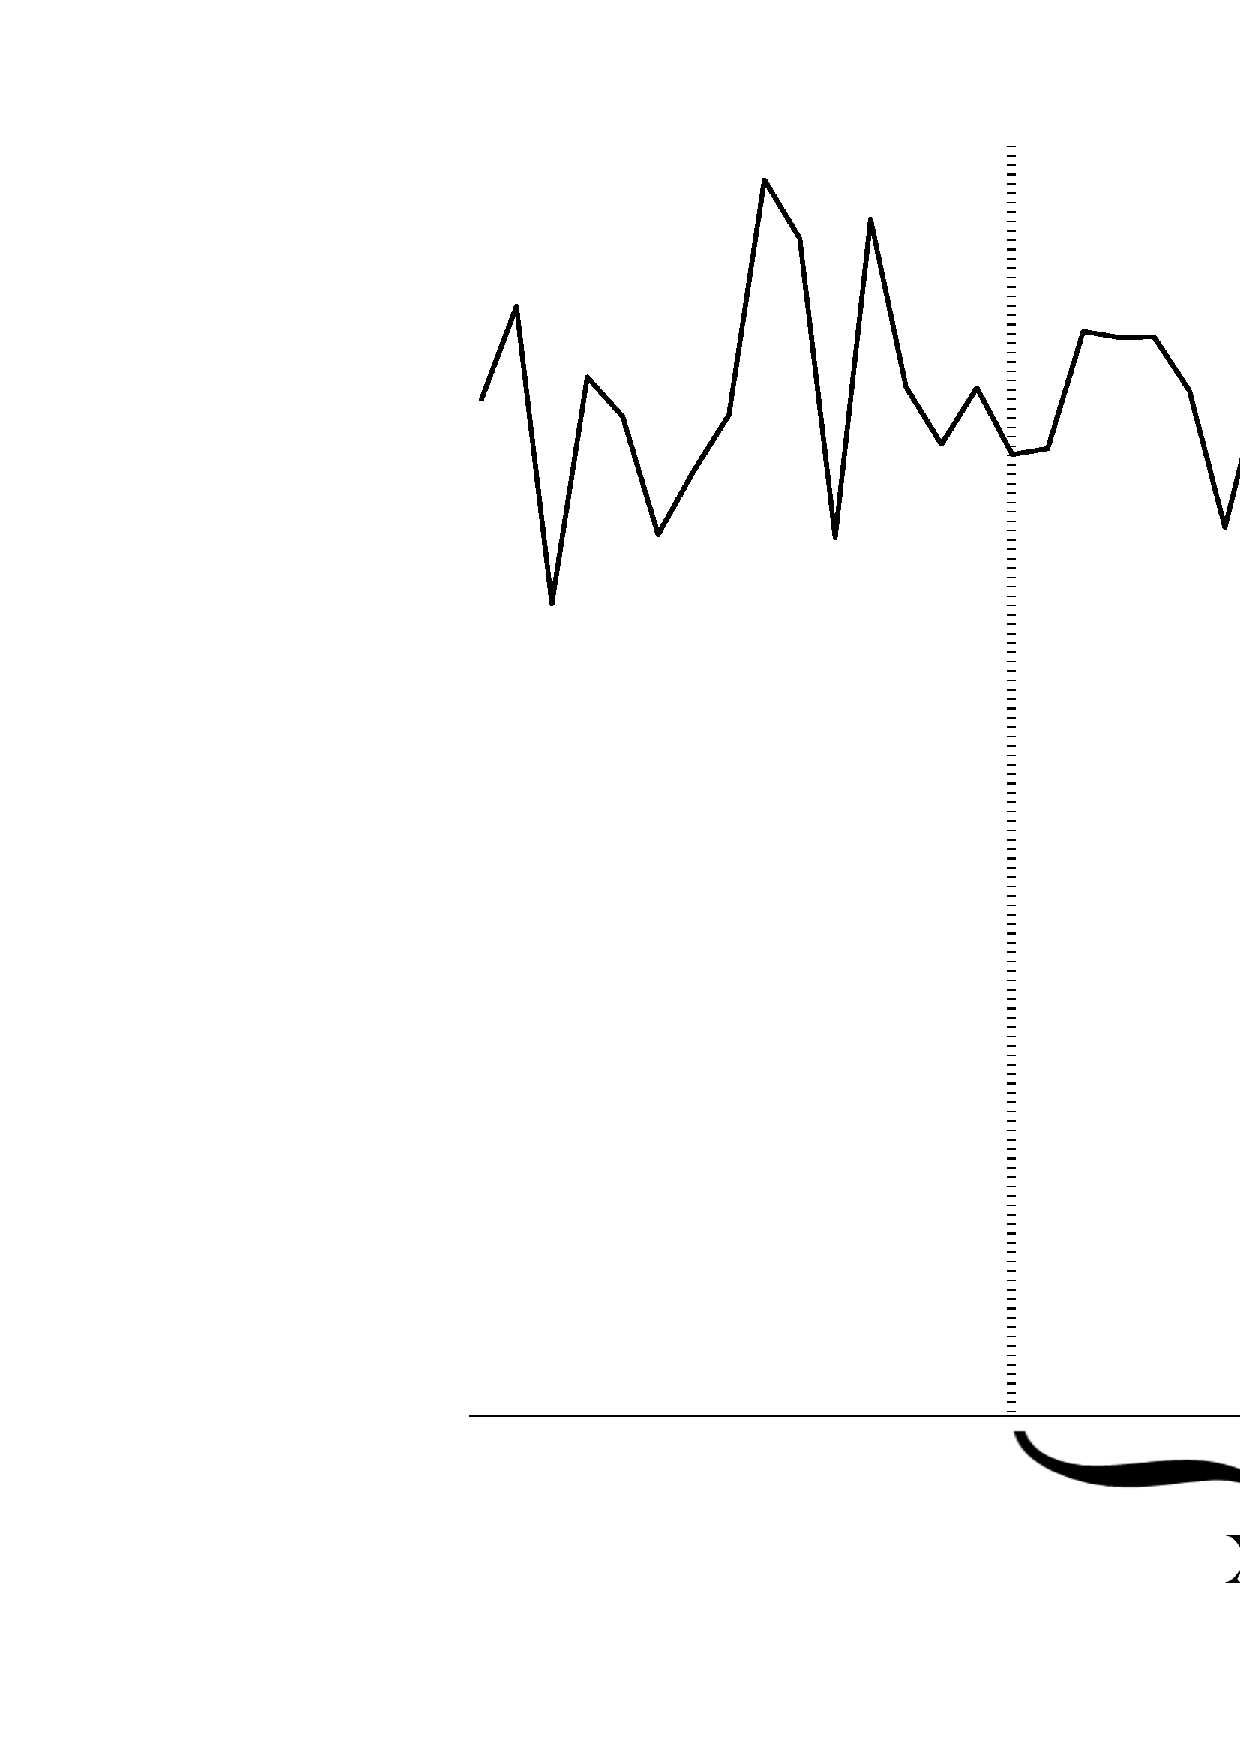
\includegraphics[scale=0.8]{cpd_ref_test.png}
 \caption{Change Point Detection}
 \label{fig:cpd_ref_test.png}
\end{figure}

Model-based approaches to change point detection assume that each tick in
a time series is a draw from some underlying probability distribution.
Scores are generated by estimating the distribution of the reference data
and the test data, and then by calculating the likelihood
that the two distributions are different.
Where it is reasonable to assume that the data belongs to a particular
family of distributions then parametric estimation methods have been employed
\cite{thatte11}. If no such modeling assumptions are reasonable then 
non-parametric methods have also been found to be viable \cite{matteson12}.
Finally, distance-based approaches such as Singular Spectrum Analysis
generate scores through other metrics of 
dissimilarity or difference between the reference data and the test data
\cite{moskvina03}.
Notationally, we say that for each tick $i$ in a time series:

\[
s_i = D(x_{r,i}, x_{t,i})
\]

Where $s_i$ is the score of the $i$th tick, $x_{r,i}$ is the reference
data associated with the $i$th tick, $x_{t,i}$ is the test data
associated with the $i$th tick, and $D(A,B)$ is a function that computes the
dissimiliarity between a matrix of data $A$ and matrix of data $B$, and is
particular to the given change point algorithm. Note that for a given
algorithm it may not be possible to generate scores right at the very beginning
of the time series (insufficient reference data) or at the very end of a time
series (insufficient test data).

\section{Methodology}

There are many different modeling assumptions and associated algorithms
for generating change point detection scores, and one simple baseline approach that we 
wanted to test was the Shewhart Control Chart. This approach assumes that the reference data is drawn from a
multivariate normal distribution, and that scores are calculated by the Mahalanobis
distance of the target time tick from the estimated multivariate normal:

\[
s_i = \sqrt{(\bar{x}_{r,i} - x_i)^T \, S_{r,i}^{-1} \, (\bar{x}_{r,i} - x_i)}
\]

where $\bar{x}_{r,i}$ is the sample mean of the reference data, $S_{r,i}$
is the sample covariance matrix of the reference data, and $x_i=x_{t,i}$ is
the $i$th data point \cite{shewhart26}.

We were also interested in testing the performance of a newer and more
sophisticated change point detection algorithm: the
Kullback-Leibler Importance Estimation Procedure (KLIEP),
introduced by Kawahara and Sugiyama \cite{sugiyama09} \cite{sugiyama08}.
This approach generates scores using the Kullback-Leibler (KL)
divergence between the reference data and the test data. One method of doing this
is to estimate the density of the reference distribution and test distribution
separately, and then compare them using a likelihood ratio
(known in the change point detection literature as \emph{importance}). 
Instead, KLIEP estimates the importance directly using a non-parametric model.

Let the estimate of the importance $\hat{R}$ be represented by this model:

\[
\hat{R} = \frac{p_{t}}{\hat{p}_{r}} = \sum_{j=1}^{n_{t}} \alpha_j K_G(x,x_{t,j})
\]

Where $p_{r}$ and $p_{t}$ are the probability densities of the reference data and the test
data, $n_{t}$ is the number of ticks in the test window, $\alpha$ is a
vector of model parameters to solve for, $x$ is the concatenation of the reference and the
test data, $x_{t,j}$ is the $j$th element of the test data,
and $K_G(A,B)$ is the Gaussian kernel with width $\sigma$:

\[
K_G(A,B) = \exp \left(-\frac{||A-B||^2}{2\sigma^2}\right)
\]

Now solve for $\alpha$ so that the empirical KL divergence between $\hat{p}_{t}$ and
$p_{t} = p_{r}\hat{R}$ is minimized, which is equivalent to the following convex optimization
problem:

\[
\begin{dcases}
 \max_{\alpha} \quad \sum_{j=1}^{n_t} \, \log \left( \sum_{k=1}^{n_t} \alpha_k K_G(x_{t,j}, x_{t,k}) \right) \\
 \,\, \text{s.t.} \quad\, \frac{1}{n_r} \sum_{j=1}^{n_r} \sum_{k=1}^{n_t} \alpha_k K_G(x_{r,j},x_{t,k}) = 1 \\
 \qquad \quad \text{and} \; \alpha_1 \ldots \alpha_{n_t} \ge 1
\end{dcases}
\]

Finally, the scores that we wish to generate are just the estimate of the importance given by the
solution to the complex optimization problem, i.e. $s_i = \hat{R}_i$.

Since this approach uses a Gaussian kernel, it requires the selection of
a kernel width $\sigma$ for each time tick. We used an implementation of
KLIEP that is available at Sugiyama's website, which included a cross-validation
procedure for the value of $\sigma$. The CV procedure chooses a number of disjoint
splits of the test data along with a number of different candidate $\sigma$'s, and runs
KLIEP with each combination of split and candidate $\sigma$. Then it chooses the candidate $\sigma$
that, on the average across all of the splits, maximizes the KL divergence (the
$\max_{\alpha}$ equation above) the most.

For the OSU Hip dataset, we used this
CV to choose the the kernel width at each individual time tick. This computationally-
intensive approach was impractical for the UQ dataset because it is orders of magnitude larger,
so instead of running it on every tick of that data, we ran the CV procedure on a number of
random ticks drawn from the data. From this we were able
to empirically identify 0.01 as a plausible $\sigma$, and so fixed $\sigma$
at that value for our experiments on this dataset.
Our reference windows were fixed at a length of 10 seconds, and our test
windows were fixed at a length of 1 second.

Once scores were generated, we chose a number of threshold values to determine which
scores were considered high enough to predict a changepoint.
Threshold values were chosen by considering the false positive rates of
change prediction for the change point detection algorithms. A smaller false positive rate
corresponded to a higher and more conservative threshold, which split the
time series into fewer segments for featurization. A larger false positive rate
corresponded to a lower threshold, which split the time series into more segments.

\section{Results}
Figure \ref{fig:cpd_perf}, shows accuracy and detection time as a function of the
false positive rate per second, for the OSU Hip dataset,
for each of the SVM, Decision Tree, and Neural Net base classifiers.

\begin{figure}
 \centering
 \includegraphics[scale=0.3]{osu_cpd_dt_acc.png}
 \includegraphics[scale=0.3]{osu_cpd_svm_acc.png}
 \includegraphics[scale=0.3]{osu_cpd_nnet_acc.png}
 \includegraphics[scale=0.3]{osu_cpd_dt_det.png}
 \includegraphics[scale=0.3]{osu_cpd_svm_det.png}
 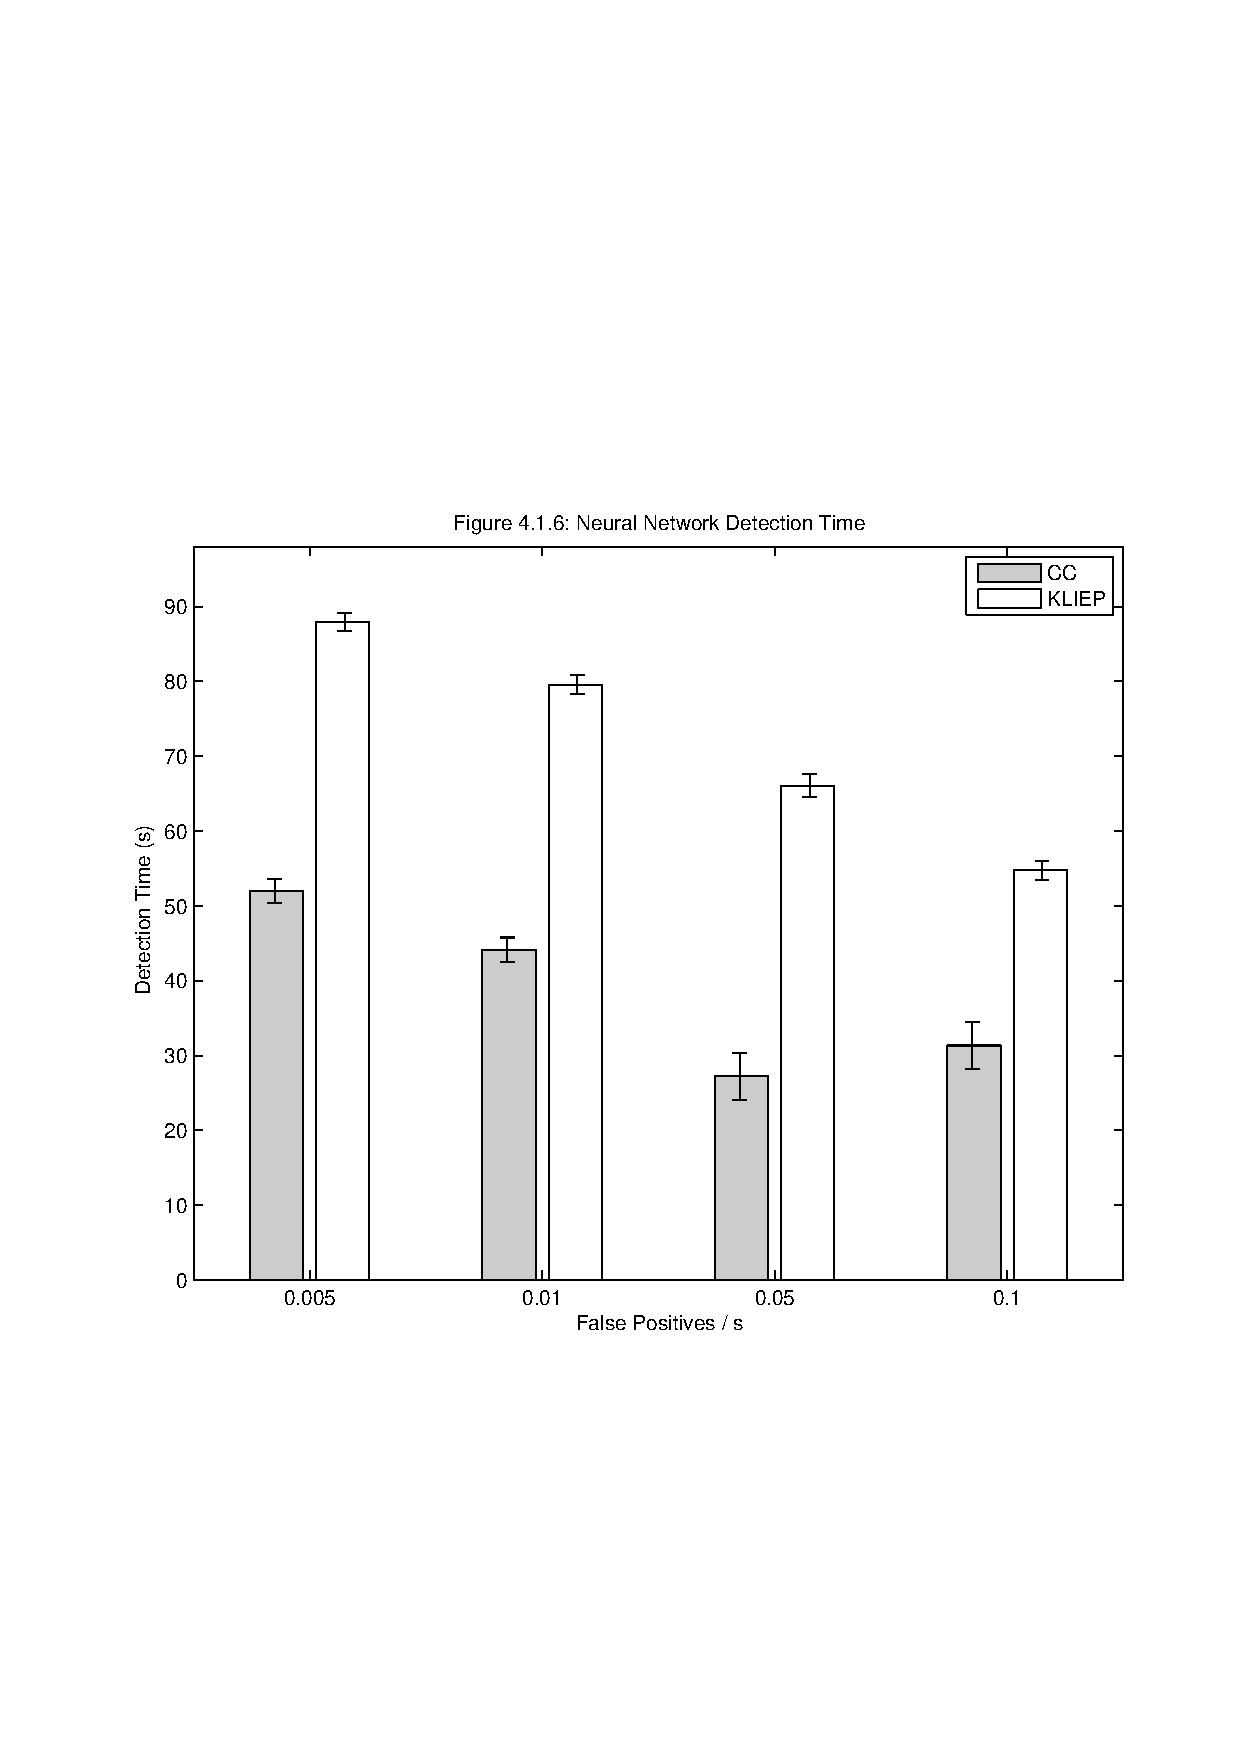
\includegraphics[scale=0.3]{osu_cpd_nnet_det.png}
 \caption{CPD-Based Classification Performance}
 \label{fig:cpd_perf}
\end{figure}

\section{Discussion}

\section{Bottom-Up Approach}
\label{sec:bottomup}




\section{Performance Metrics}
To measure the performance of our classification algorithms we used
two metrics. Accuracy is defined as the number of ticks that an algorithm
correctly classifies in a time series, over the total number of ticks
in the time series. Since we were also interested in our algorithms'
feasibility for activity classification in real time, we used detection time as
a second metric. Detection time is defined as the average amount of time
required for an algorithm to begin correctly classifying data after a
true activity change has occurred.

In the change-point detection experiments accuracy and detection time were
averaged over 30 random splits of the given dataset into training, validation, and
testing sets. Because the HMM experiments were more computationally
expensive, accuracy and detection time were averaged over 10 random splits of
the given dataset into training (base classifier), validation, training (HMM),
and testing sets.

\chapter{Results}
%Figure \ref{fig:cpd_perf}, shows accuracy and detection time as a function of the
%false positive rate per second, for the OSU Hip dataset,
%for each of the SVM, Decision Tree, and Neural Net base classifiers.
%
%\begin{figure}
% \centering
% \includegraphics[scale=0.3]{osu_cpd_dt_acc.png}
% \includegraphics[scale=0.3]{osu_cpd_svm_acc.png}
% \includegraphics[scale=0.3]{osu_cpd_nnet_acc.png}
% \includegraphics[scale=0.3]{osu_cpd_dt_det.png}
% \includegraphics[scale=0.3]{osu_cpd_svm_det.png}
% 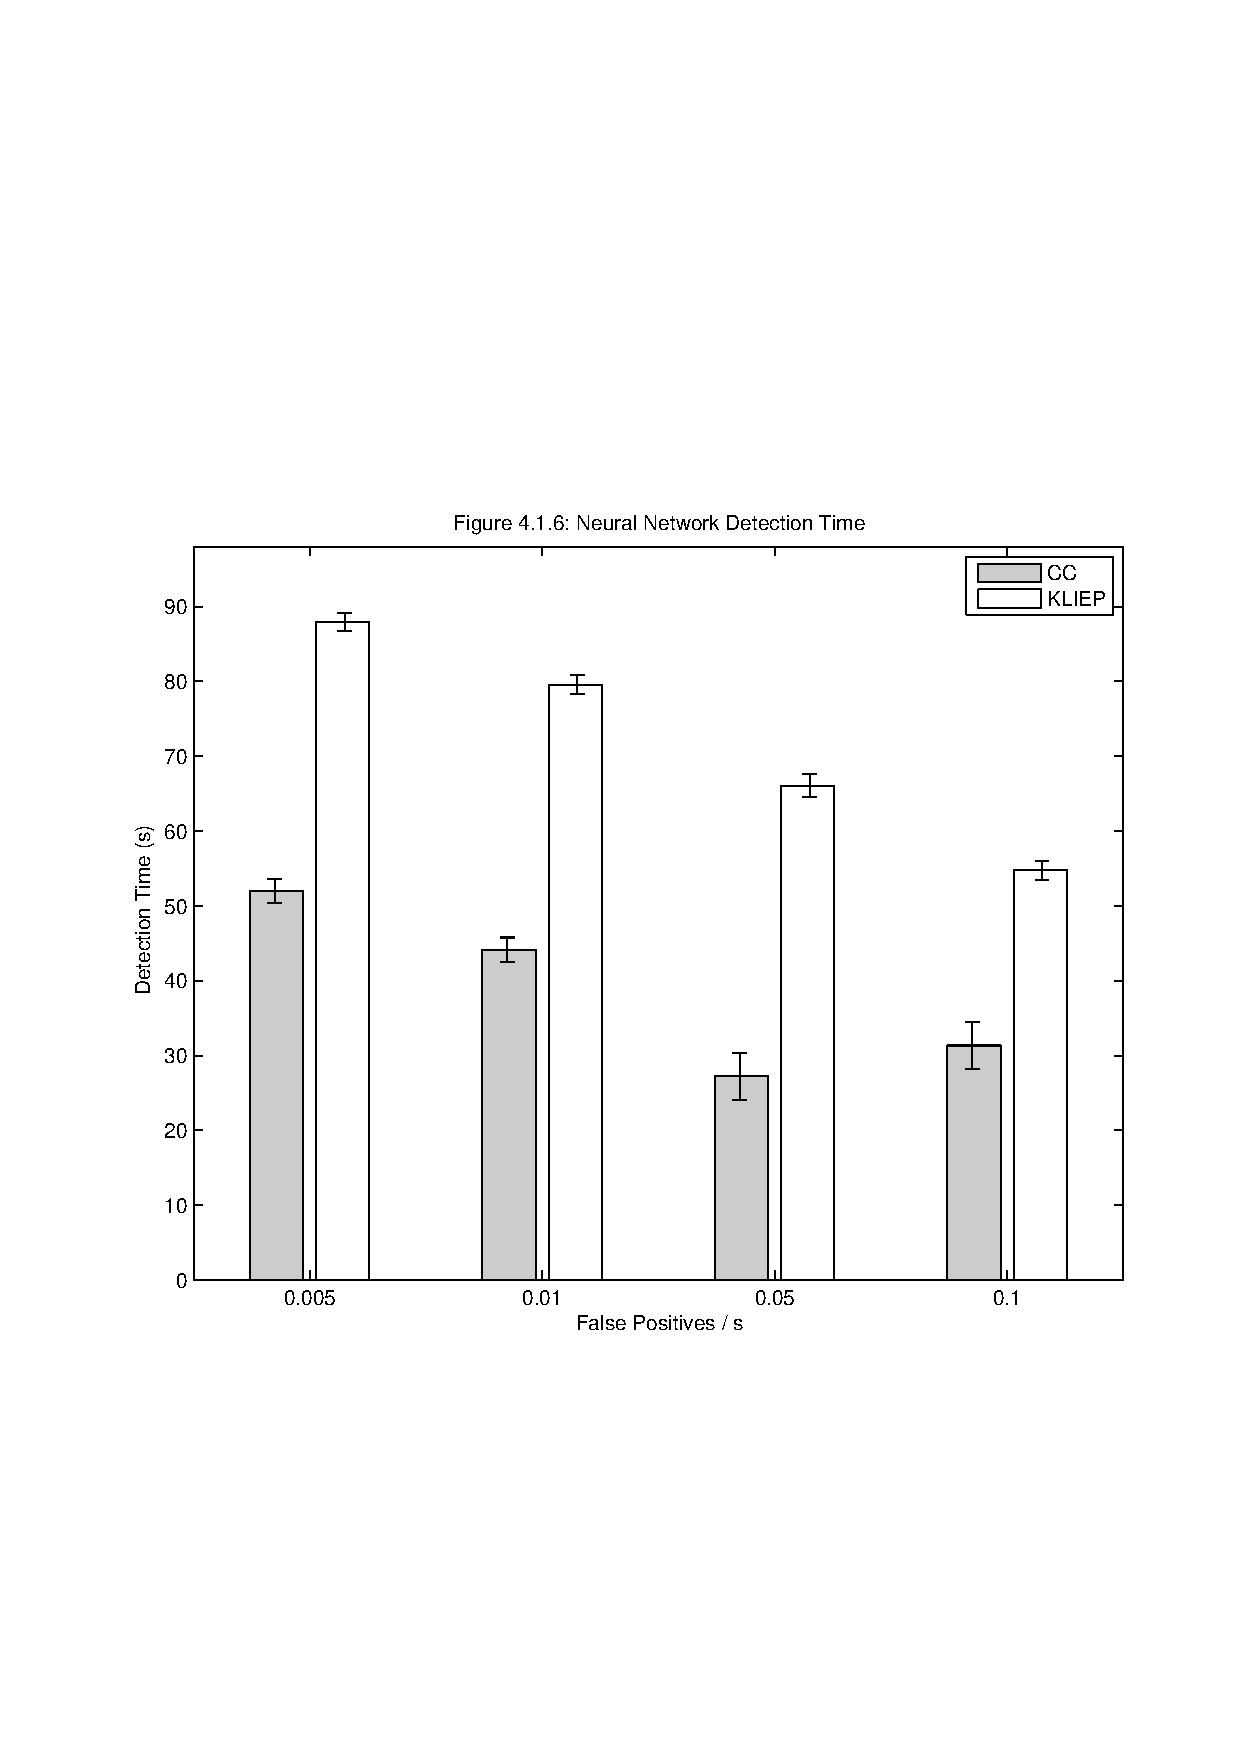
\includegraphics[scale=0.3]{osu_cpd_nnet_det.png}
% \caption{CPD-Based Classification Performance}
% \label{fig:cpd_perf}
%\end{figure}

\section{Change-Point Detection}
Results for our change-point detection experiments are given in
Figures \ref{fig:osu_cpd}-\ref{fig:lime2_cpd}.
We hypothesized that the performance of the change-point detection algorithms
would depend heavily on the threshold level for change prediction. This was
tested by varying the average number of times per second that the algorithms
falsely predicted a change. A large number of such false positive rates per
second were tested, but for the sake of brevity only a representative sample
of $\{0.005, 0.01, 0.05, 0.1\}$ are shown here.

In the OSU Hip experiments, control charts outperformed KLIEP in terms of
detection time (Figures 4.1.2, 4.1.4, 4.1.6), while the accuracy results were
mixed. It is generally expected that the accuracy curve as
a function of the false positive rate will be unimodal: very large windows
extend into multiple activities and confuse a classifier, while very small
windows do not contain enough information to be discriminative. This
unimodal behavior is shown in the control chart results, but not in the KLIEP
results (Figures 4.1.1, 4.1.3, 4.1.5). Follow-up experiments showed that the peak
in KLIEP accuracy performance occurred between false positive rates of $0.2$ and
$0.3$ for each of the three classifiers.

Further investigation indicated that across the OSU Hip dataset the KLIEP algorithm
was unable to detect many different activity changes without a very low score
threshold value (and consequently very high false positive rates).
Some qualitative plotting of the OSU Hip data showed
that most of its activities have accelerometer amplitude values that strongly
resemble draws from a multivariate normal distribution. Since control charts
assume that the data is drawn from a distribution that is a member of that
family, it is logical that control charts would outperform algorithms with
different modeling assumptions on OSU Hip.

In the LiME experiments, KLIEP outperformed control charts in terms of
accuracy across the board, and control charts outperformed KLIEP in terms of
detection time across the board. (TODO: Need to interpret this, but not sure
how.)

Finally, in a few cases (Figures 4.1.2, 4.1.6, 4.2.6) the detection time did
not decrease as the false positive rate increased. On the face of it this would seem
to be a non-sequitur, but this only happened in cases when accuracy also decreased
(Figures 4.1.1, 4.1.5, 4.2.5).
Smaller window sizes tend to be correlated with decreased detection times, but
it is possible that predicting on smaller windows, if they happen to be less discriminative,
can actually increase the time required for the classifier to start correctly
predicting the ground-truth activity. Additionally, the given increases in detection
time were small and near standard error.

%\setlength{\abovecaptionskip}{-5pt}

\begin{table}[h]
\captionsetup{font=scriptsize}
\begin{center}
\tiny{
\begin{tabular}{ cc|c|c|c|c|c|c|c|c|c|c|c|c| }
\cline{3-14}
& & \multicolumn{4}{ c| }{DT} & \multicolumn{4}{ c| }{SVM} & \multicolumn{4}{ c| }{NNET}\\ \cline{3-14}
& & 0.005 & 0.01 & 0.05 & 0.1 & 0.005 & 0.01 & 0.05 & 0.1 & 0.005 & 0.01 & 0.05 & 0.1\\ \cline{1-14}
\multicolumn{1}{ |c| }{\multirow{2}{*}{OSU Hip}} &
\multicolumn{1}{ |c| }{CC} & 49.2 & 46.8 & 38.9 & 35.4 & 66.8 & \textbf{67.9} & 55.2 & 47.0 & 62.3 & 65.9 & 64.5 & 53.1\\ \cline{2-14}
\multicolumn{1}{ |c }{} &
\multicolumn{1}{ |c| }{KLIEP} & 31.0 & 32.3 & 36.9 & 41.3 & 40.3 & 44.3 & 52.1 & 58.0 & 41.0 & 43.8 & 53.0 & \textbf{59.9}\\ \cline{1-14}
\multicolumn{1}{ |c| }{\multirow{2}{*}{LiME Day 1}} &
\multicolumn{1}{ |c| }{CC} & 47.5 & 48.2 & 43.0 & 41.9 & \textbf{57.7} & 57.3 & 52.0 & 51.4 & 19.1 & 21.0 & 17.4 & 16.8\\ \cline{2-14}
\multicolumn{1}{ |c }{} &
\multicolumn{1}{ |c| }{KLIEP} & 58.8 & 57.6 & 53.8 & 52.3 & \textbf{68.7} & 66.7 & 61.9 & 59.2 & 23.6 & 20.8 & 22.9 & 19.0\\ \cline{1-14}
\multicolumn{1}{ |c| }{\multirow{2}{*}{LiME Day 2}} &
\multicolumn{1}{ |c| }{CC} & \textbf{54.0} & 53.6 & 50.3 & 50.2 & 53.3 & 52.5 & 49.5 & 45.9 & 21.6 & 19.7 & 17.3 & 15.4\\ \cline{2-14}
\multicolumn{1}{ |c }{} &
\multicolumn{1}{ |c| }{KLIEP} & 63.4 & 61.5 & 59.0 & 58.6 & \textbf{65.5} & 63.2 & 58.1 & 55.8 & 25.6 & 20.0 & 20.1 & 19.6\\ \cline{1-14}
\end{tabular}
}
\end{center}
\caption{CPD Accuracy}
\label{tbl:cpd_acc}
\end{table}

\begin{table}[h]
\captionsetup{font=scriptsize}
\begin{center}
\tiny{
\begin{tabular}{ c|c|c|c|c|c|c| }
\cline{2-7}
 & \multicolumn{2}{ c| }{DT} & \multicolumn{2}{ c| }{SVM} & \multicolumn{2}{ c| }{NNET}\\ \cline{2-7}
 & 20 & 10 & 20 & 10 & 20 & 10\\ \cline{1-7}
\multicolumn{1}{ |c| }{OSU Hip}
 & 89.5 & 88.1 & \textbf{94.9} & 94.4 & 71.2 & 62.2\\ \cline{1-7}
\multicolumn{1}{ |c| }{LiME Day 1}
 & 84.3 & 83.3 & 78.3 & \textbf{84.8} & 69.6 & 51.7\\ \cline{1-7}
\multicolumn{1}{ |c| }{LiME Day 2}
 & \textbf{87.5} & 85.6 & 79.4 & 86.4 & 57.7 & 78.4\\ \cline{1-7}
\end{tabular}
}
\end{center}
\caption{HMM Accuracy}
\label{tbl:hmm_acc}
\end{table}

\begin{table}[h]
\captionsetup{font=scriptsize}
\begin{center}
\tiny{
\begin{tabular}{ cc|c|c|c|c|c|c|c|c|c|c|c|c| }
\cline{3-14}
& & \multicolumn{4}{ c| }{DT} & \multicolumn{4}{ c| }{SVM} & \multicolumn{4}{ c| }{NNET}\\ \cline{3-14}
& & 0.005 & 0.01 & 0.05 & 0.1 & 0.005 & 0.01 & 0.05 & 0.1 & 0.005 & 0.01 & 0.05 & 0.1\\ \cline{1-14}
\multicolumn{1}{ |c| }{\multirow{2}{*}{OSU Hip}} &
\multicolumn{1}{ |c| }{CC} & 69.7 & 66.5 & 68.8 & 70.7 & 49.3 & 42.2 & 35.9 & 35.0 & 52.0 & 44.2 & \textbf{27.2} & 31.3\\ \cline{2-14}
\multicolumn{1}{ |c }{} &
\multicolumn{1}{ |c| }{KLIEP} & 101.6 & 98.9 & 94.0 & 88.5 & 87.1 & 81.6 & 71.8 & 63.3 & 86.9 & 78.6 & 65.1 & \textbf{53.8}\\ \cline{1-14}
\multicolumn{1}{ |c| }{\multirow{2}{*}{LiME Day 1}} &
\multicolumn{1}{ |c| }{CC} & 107.2 & 76.9 & 56.0 & 51.3 & 79.1 & 55.5 & 36.6 & \textbf{32.8} & 168.8 & 111.1 & 78.2 & 76.8\\ \cline{2-14}
\multicolumn{1}{ |c }{} &
\multicolumn{1}{ |c| }{KLIEP} & 146.1 & 116.0 & 59.7 & 50.9 & 113.5 & 88.7 & 43.8 & \textbf{36.0} & 237.9 & 191.4 & 92.5 & 82.3\\ \cline{1-14}
\multicolumn{1}{ |c| }{\multirow{2}{*}{LiME Day 2}} &
\multicolumn{1}{ |c| }{CC} & 103.7 & 80.4 & 59.8 & 54.3 & 101.8 & 72.2 & 52.1 & \textbf{48.8} & 161.5 & 130.2 & 78.6 & 72.0\\ \cline{2-14}
\multicolumn{1}{ |c }{} &
\multicolumn{1}{ |c| }{KLIEP} & 136.0 & 121.3 & 63.2 & 54.8 & 127.3 & 112.3 & 58.4 & \textbf{50.4} & 242.6 & 216.6 & 109.2 & 88.3\\ \cline{1-14}
\end{tabular}
}
\end{center}
\caption{CPD Detection Time}
\label{tbl:cpd_det}
\end{table}

\begin{table}[h]
\captionsetup{font=scriptsize}
\begin{center}
\tiny{
\begin{tabular}{ c|c|c|c|c|c|c| }
\cline{2-7}
 & \multicolumn{2}{ c| }{DT} & \multicolumn{2}{ c| }{SVM} & \multicolumn{2}{ c| }{NNET}\\ \cline{2-7}
 & 20 & 10 & 20 & 10 & 20 & 10\\ \cline{1-7}
\multicolumn{1}{ |c| }{OSU Hip}
 & 9.8 & 9.8 & 4.5 & \textbf{4.2} & 31.4 & 40.1\\ \cline{1-7}
\multicolumn{1}{ |c| }{LiME Day 1}
 & 57.1 & 32.2 & 103.5 & \textbf{25.0} & 177.7 & 146.3\\ \cline{1-7}
\multicolumn{1}{ |c| }{LiME Day 2}
 & 47.8 & \textbf{31.7} & 101.2 & 31.8 & 255.5 & 53.7\\ \cline{1-7}
\end{tabular}
}
\end{center}
\caption{HMM Detection Time}
\label{tbl:hmm_det}
\end{table}

\setlength{\abovecaptionskip}{10pt}


\begin{figure}[H]
 \includegraphics[scale=0.4]{osu_cpd_dt_acc.pdf} \hspace{1em}\vspace{1em}
 \includegraphics[scale=0.4]{osu_cpd_dt_det.pdf}
 \includegraphics[scale=0.4]{osu_cpd_svm_acc.pdf} \hspace{1em}\vspace{1em}
 \includegraphics[scale=0.4]{osu_cpd_svm_det.pdf}
 \includegraphics[scale=0.4]{osu_cpd_nnet_acc.pdf} \hspace{2em}
 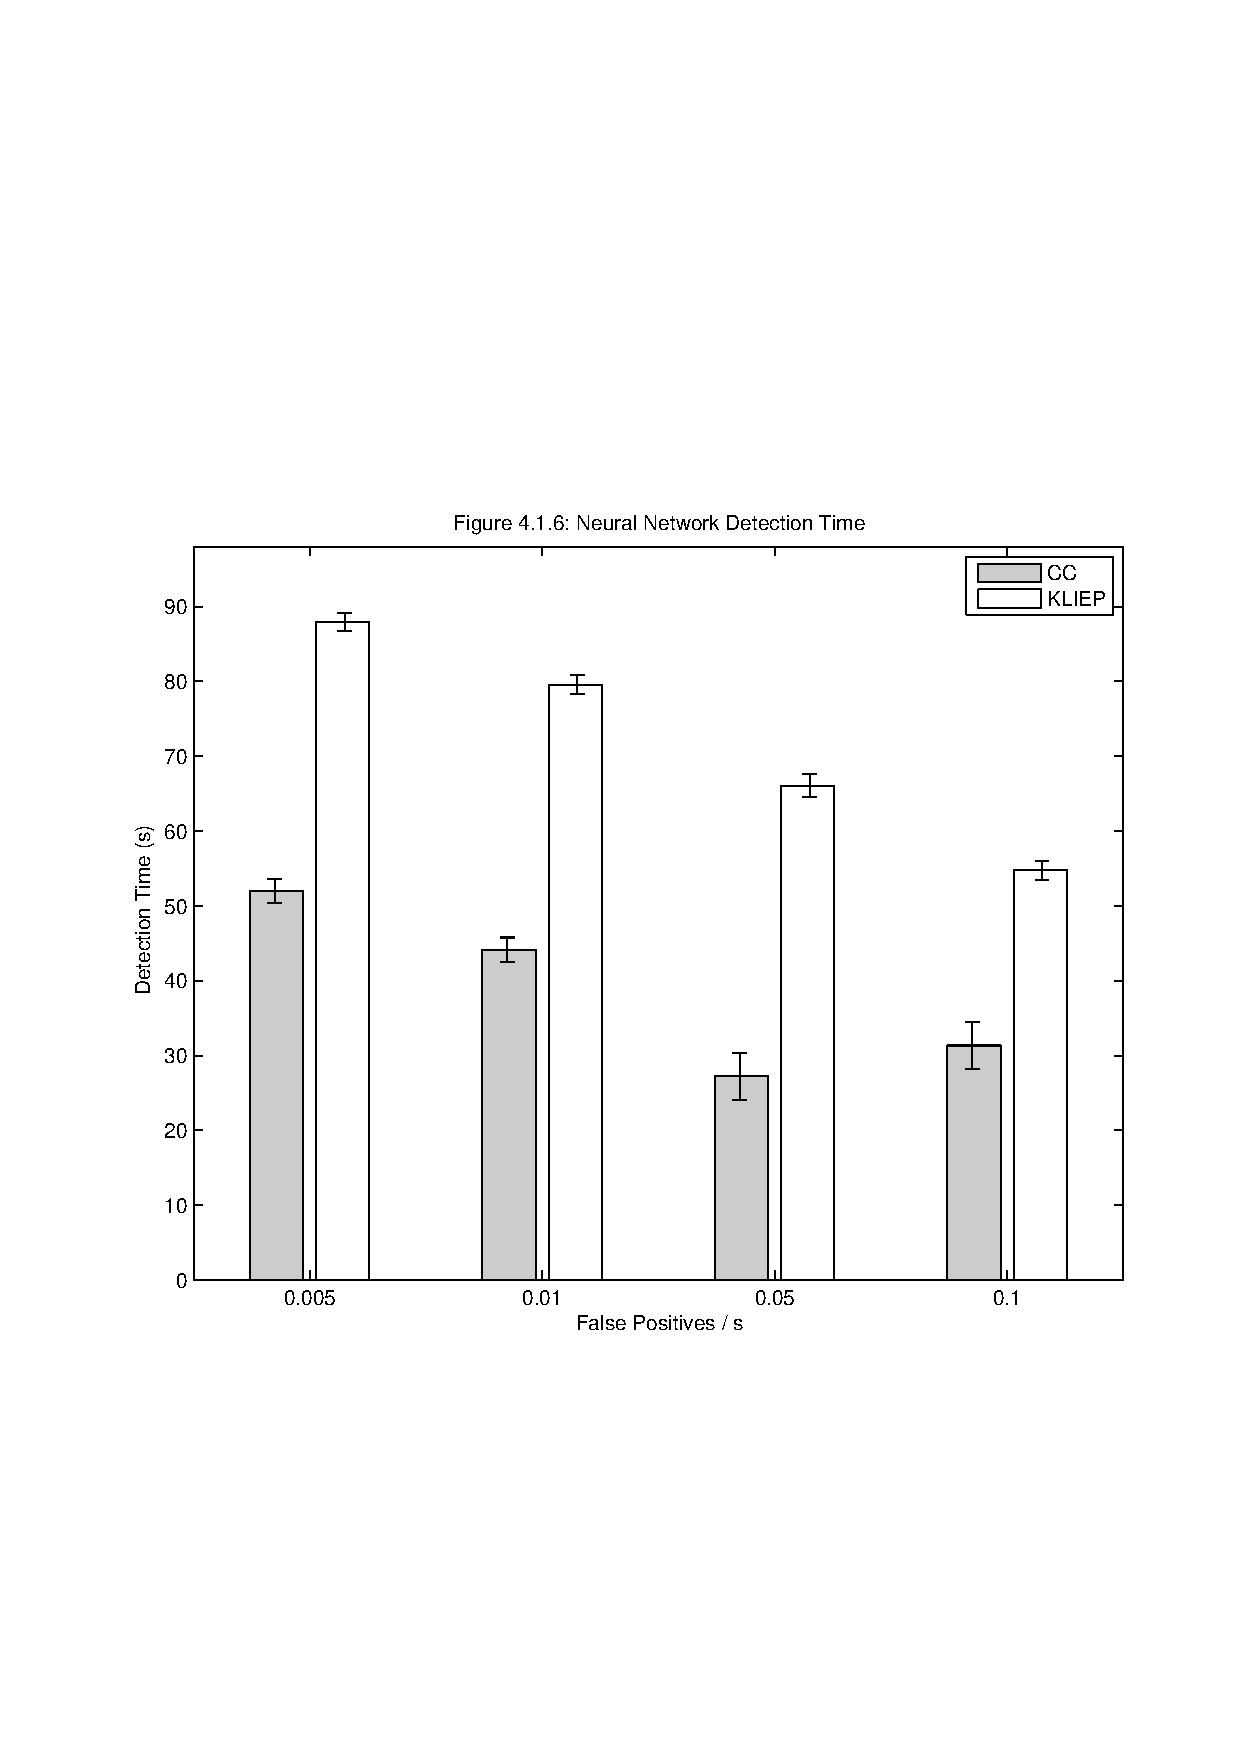
\includegraphics[scale=0.4]{osu_cpd_nnet_det.pdf}
 \caption{OSU Hip Results. Graphs are organized into rows by base classifier,
  and columns by evaluation metric. Change-point detection result were averaged over
  30 splits into training, testing, and validation datasets,
  along with bars showing one standard error.}
 \label{fig:osu_cpd}
\end{figure}

\begin{figure}[H]
 \centering
 \includegraphics[scale=0.4]{lime1_cpd_dt_acc.pdf} \hspace{1em}\vspace{1em}
 \includegraphics[scale=0.4]{lime1_cpd_dt_det.pdf}
 \includegraphics[scale=0.4]{lime1_cpd_svm_acc.pdf} \hspace{1em}\vspace{1em}
 \includegraphics[scale=0.4]{lime1_cpd_svm_det.pdf}
 \includegraphics[scale=0.4]{lime1_cpd_nnet_acc.pdf} \hspace{1em}
 \includegraphics[scale=0.4]{lime1_cpd_nnet_det.pdf}
 \caption{LiME Day 1 Results}
 \label{fig:lime1_cpd}
\end{figure}

\begin{figure}[H]
 \centering
 \includegraphics[scale=0.4]{lime2_cpd_dt_acc.pdf} \hspace{1em}\vspace{1em}
 \includegraphics[scale=0.4]{lime2_cpd_dt_det.pdf}
 \includegraphics[scale=0.4]{lime2_cpd_svm_acc.pdf} \hspace{1em}\vspace{1em}
 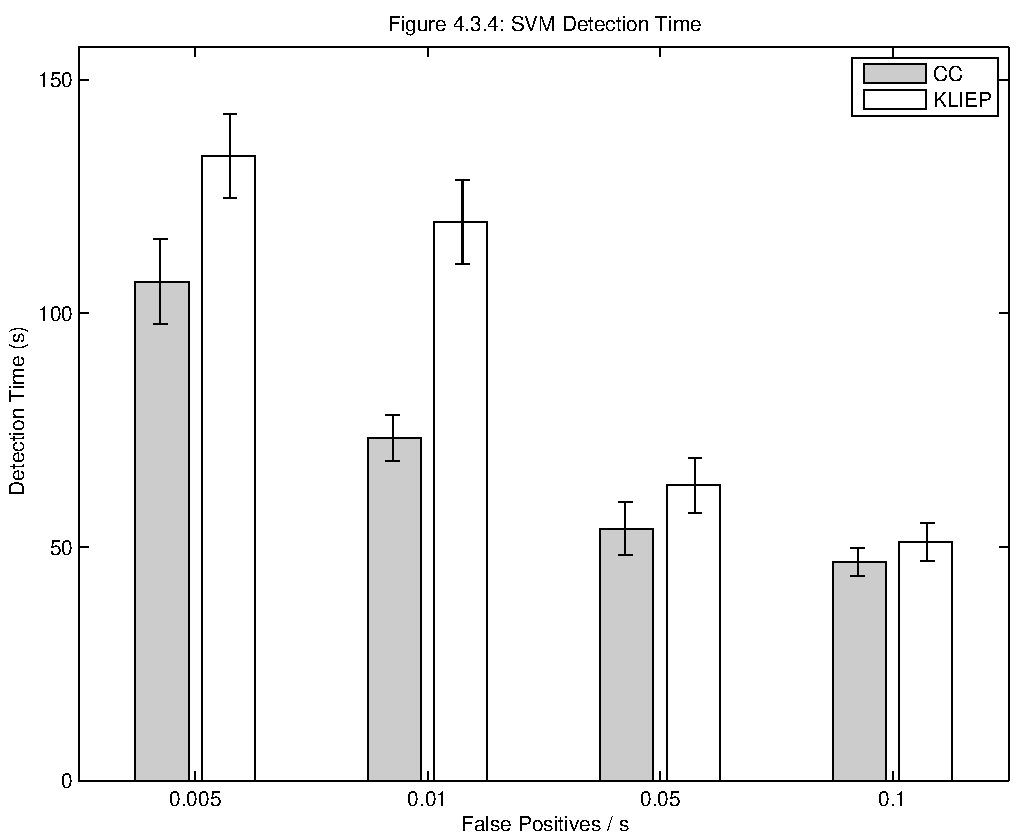
\includegraphics[scale=0.4]{lime2_cpd_svm_det.pdf}
 \includegraphics[scale=0.4]{lime2_cpd_nnet_acc.pdf} \hspace{1em}
 \includegraphics[scale=0.4]{lime2_cpd_nnet_det.pdf}
 \caption{LiME Day 2 Results}
 \label{fig:lime2_cpd}
\end{figure}


\section{HMM}

Results for our HMM experiments are given in
Figures \ref{fig:osu_hmm}-\ref{fig:lime2_hmm}. Each HMM experiment was
performed by splitting time series into windows of fixed length for
featurization, and results for windows of length $\{10, 12, 14, 16, 18, 20\}$
seconds are shown.

For both the SVM and decision tree classifiers, accuracy and detection time
was strong across all three datasets, and also stable with respect to window
size. Further experiments on the OSU Hip dataset showed that the HMM when
paired with these classifiers
tends to be stable with window sizes that are greater than a few seconds,
which seems to be the amount of time required to be informative. Neural networks
performed somewhat more poorly and erratically across the board.

\begin{figure}[H]
 \centering
 \includegraphics[scale=0.4]{osu_hmm_dt_acc.pdf} \hspace{1em}\vspace{1em}
 \includegraphics[scale=0.4]{osu_hmm_dt_det.pdf}
 \includegraphics[scale=0.4]{osu_hmm_svm_acc.pdf} \hspace{1em}\vspace{1em}
 \includegraphics[scale=0.4]{osu_hmm_svm_det.pdf}
 \includegraphics[scale=0.4]{osu_hmm_nnet_acc.pdf} \hspace{1em}
 \includegraphics[scale=0.4]{osu_hmm_nnet_det.pdf}
 \caption{OSU Hip HMM Results.
  Graphs are organized into rows by base classifier, and columns by evaluation
  metric. HMM results were averaged over 10 splits into training
  (base classifier), validation, training (HMM), and testing datasets, along with bars
  showing one standard error.}
 \label{fig:osu_hmm}
\end{figure}

\begin{figure}[H]
 \centering
 \includegraphics[scale=0.4]{lime1_hmm_dt_acc.pdf} \hspace{1em}\vspace{1em}
 \includegraphics[scale=0.4]{lime1_hmm_dt_det.pdf} 
 \includegraphics[scale=0.4]{lime1_hmm_svm_acc.pdf} \hspace{1em}\vspace{1em}
 \includegraphics[scale=0.4]{lime1_hmm_svm_det.pdf} 
 \includegraphics[scale=0.4]{lime1_hmm_nnet_acc.pdf} \hspace{1em}
 \includegraphics[scale=0.4]{lime1_hmm_nnet_det.pdf} 
 \caption{LiME Day 1 HMM Results}
 \label{fig:lime1_hmm}
\end{figure}

\begin{figure}[H]
 \centering
 \includegraphics[scale=0.4]{lime2_hmm_dt_acc.pdf} \hspace{1em}\vspace{1em}
 \includegraphics[scale=0.4]{lime2_hmm_dt_det.pdf}
 \includegraphics[scale=0.4]{lime2_hmm_svm_acc.pdf} \hspace{1em}\vspace{1em}
 \includegraphics[scale=0.4]{lime2_hmm_svm_det.pdf}
 \includegraphics[scale=0.4]{lime2_hmm_nnet_acc.pdf} \hspace{1em}
 \includegraphics[scale=0.4]{lime2_hmm_nnet_det.pdf}
 \caption{LiME Day 2 HMM Results}
 \label{fig:lime2_hmm}
\end{figure}

\newpage

\section{Discussion}

Our results clearly show that the HMM approach outperformed the change-point
detection approach, both in terms of accuracy and detection time, regardless of
the dataset and base classifier. This was expected, as our change-point
detection algorithms did not perform expecially well at predicting changes at
the correct locations, and also because HMMs are a well-established and well-
grounded approach in sequential, time-oriented domains.

A further point of interest was that SVM clearly beat out the other two
base classifiers, and that the faster and simpler decision tree model did fairly
well against neural networks. This result is significant because much of the
previous research that has formulated activity detection as a supervised learning
problem has used neural networks exclusively.

\chapter{Conclusion}
The purpose of this work was to test the feasibility of using change-point
detection techniques for deciding when one activity ended within a time series
and the next began, and to contrast this technique with an HMM approach.
The bottom-up approach clearly outperformed
the top-down approach. We also showed that the performance of a change-point
detection algorithm was highly dependent on how well the data fit the modeling
assumption of the algorithm, so it is plausible that a change-point detection
algorithm with a modeling assumption that is in accord with the given data will
perform well.


\bibliographystyle{plain}
\bibliography{thesis}

%\appendix
%\chapter{Redundancy}
%This appendix is inoperable.
%
\end{document}
